% vim: set tw=78 sts=2 sw=2 ts=8 aw et ai:
\documentclass[12pt]{article}

\usepackage[paper=a4paper, top=2cm, bottom=3cm, left=2.5cm, right=2.5cm]{geometry}

\usepackage{ucs}
\usepackage[utf8x]{inputenc}
\usepackage[english]{babel}
%\usepackage{hyperref}	  % use \url{http://$URL} or \href{http://$URL}{Name}
\usepackage{underscore}	  % underscores need not be escaped
\usepackage{subfigure}
\usepackage{verbatim}
\usepackage{float}
\usepackage{booktabs}     % professional tables

% Support for including graphics
\usepackage{graphicx}
\DeclareGraphicsExtensions{.pdf,.png,.jpg}

\usepackage{color}
\usepackage{listings}
\lstset{ %
language=C++,                % choose the language of the code
basicstyle=\footnotesize,       % the size of the fonts that are used for the code
numbers=left,                   % where to put the line-numbers
numberstyle=\footnotesize,      % the size of the fonts that are used for the line-numbers
stepnumber=1,                   % the step between two line-numbers. If it is 1 each line will be numbered
numbersep=5pt,                  % how far the line-numbers are from the code
backgroundcolor=\color{white},  % choose the background color. You must add \usepackage{color}
showspaces=false,               % show spaces adding particular underscores
showstringspaces=false,         % underline spaces within strings
showtabs=false,                 % show tabs within strings adding particular underscores
frame=single,           % adds a frame around the code
tabsize=2,          % sets default tabsize to 2 spaces
captionpos=b,           % sets the caption-position to bottom
breaklines=true,        % sets automatic line breaking
breakatwhitespace=false,    % sets if automatic breaks should only happen at whitespace
escapeinside={\%*}{*)}          % if you want to add a comment within your code
}

\title{Hive - Wireless Sensor Networks simulator}

\author{Catalina Macalet, Sorin Dumitru\\
Automatic Control and Computers Faculty\\
University POLITEHNICA of Bucharest\\
Splaiul Independenței nr. 313, Bucharest, Romania \\
\emph{\{catalina.macalet,sorin.dumitru\}@cs.pub.ro}}

\date{\today}

\begin{document}

\maketitle

\begin{abstract}
% vim: set tw=78 sts=2 sw=2 ts=8 aw et ai:
This paper describes Hive, a Wireless Sensor Nodes network simulator.
Hive is component based and highly scalable allowing simulations
of thousands of nodes.

It provides a standard library based on events for developing applications
for Wireless Sensor Nodes. It abstracts architecture, network protocols and
components in order to provide portability.

\end{abstract}

\section{Introduction}
\label{sec:introduction}
% vim: set tw=78 sts=2 sw=2 ts=8 aw et ai:
\textit{Hive} is a Wireless Sensor Network Simulator that is intended to be
used for simulating routing protocols for Wireless Sensors Networks in order
to determine the best suited protocol for a given topology.
There exist a number of simulators used for simulating Wireless Sensor
Networks such as NS-2, J-sim\cite{jsim-article} and TOSSIM\cite{tossim}. We will not go into details regarding
these simulator since this was covered in our previous work. What is to be
noted though is that, after the survey we did on these simulators, we were able
to define some key features that we wanted the \textit{Hive} simulator to
have, such as, but not limited to: to be component based in order to make it easy to extend and to make future development easier to
be done, to be able to simulate a wide variety of nodes in order to not be
limited to only some sensors types, to make it easy to write code that is to
be run on nodes in order to make the implementation of the routing protocols
easier to be done and, after looking at the trends in the Wireless Sensor
Networks research, we decided that the simulator should, in the begining
support at least the 6LoWPAN and ZigBee protocol stacks.
Also, unlike some of the simulators enumerated above, \textit{Hive} targets topologies of Wireless Sensor
Networks and so, during the desing and implementation phases decisions were
made so that \textit{Hive} could simulate as accurate as possible a real
sensor.

The structure of the paper is at follows: in section 2 we present the
\textit{Architecture} of the \textit{Hive} simulator, discussing the reasons for which such
an architecture was chosen and present the communication mechanisms between
the components. Then, the \textit{Implementation} section follows where we briefly present
the libraries and tools used for implementation and the reasons for which we
chose to use these and, also, go into some details concerning the implementation.
In section \textit{Testing} we present the tests we want to do in
order to test the way \textit{Hive} behaves and to be able to provide some
numbers for the scalability matter.
In the end some conclusions are drawn, and the next steps are highlighted in
the \textit{Conclusions and Further Work} section. 


\section{Architecture}
\label{sec:architecture}
% vim: set tw=78 sts=2 sw=2 ts=8 aw et ai:

\begin{figure}[htb]
  \begin{center}
    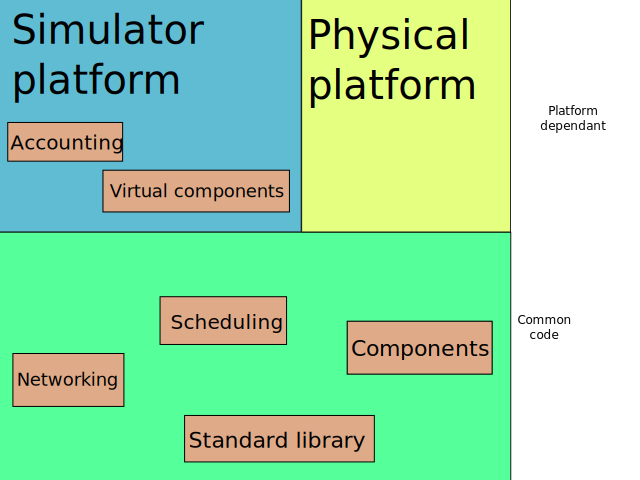
\includegraphics[scale=0.75]{img/bigarch.pdf}
    \caption{Hive simulator Architecture}
  \end{center}
\end{figure}


\subsection{Controlling the simulator}

The simulator is controlled through simple commands on a TCP socket. For
example to load a test plugin, start it, stop it and then unload it we would
do:
\begin{lstlisting}
$ nc 127.0.0.1 54321
load test
1
start 1
stop 1
unload 1
\end{lstlisting}
If the library test.so is not found in LD_LIBRARY_PATH an error will be
thrown.


\section{Implementation}
\label{sec:implementation}
% vim: set tw=78 sts=2 sw=2 ts=8 aw et ai:

\subsection{Standard library}

In order for the wireless sensor nodes to be usefull they will have to be
programmed to do a certain task. For this, Hive provides an API. It allows
common tasks like scheduling a timer or creating sockets. 

This API provided by Hive is platform agnostic. The code is loadable in the
simulator as plugin using libdl. When used on a physical node, the plugin must
provide only a load rutine. When ran on the simulator platform, the plugin
should also provide a start, stop and unload rutine.

\subsection{Networking}

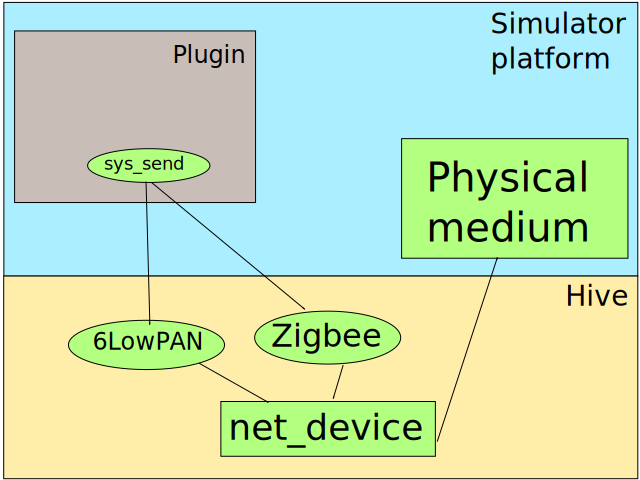
\includegraphics[scale=0.75]{img/networking.pdf}

\subsection{Scheduler}

Most of work on a wireless sensor node is triggered by an event. For example
we read the temperature sensor every 5 minutes, which is a timer event, or an
actual event happens on the node, for example a packet arrives.

The job of the scheduler is to provide a way to register for and notify of
events. It's split into two parts, a platform agnostic one and a platform
specific one. The platform agnostic part contains the API for users to use the
scheduler. It allows specifing callback for events or timers:

\begin{lstlisting}
typedef void (*callback_t)(void *arg);
void schedule_timer(struct scheduler *scheduler,
                    /* Timeout in miliseconds *?
                    int timeout, 
                    /* Callback function */
                    callback_t *cb, 
                    /* Argument to be passed to the callback */
                    void *arg);
\end{lstlisting}
The platform specific part contains the platform dependent implementation of
the scheduler. Each platform has a different implementation for timers so each
platform will have to implement its own version of this. For example linux has
timerfds, but an Atmega microcontroller has hardware timers. The scheduler
implementation for that platform will use what the platform provides.

The implementation of the scheduler on the simulation platform will be done
using libevent. The libevent API provides a mechanism to execute a callback
function when a specific event occurs on a file descriptor or after a timeout
has been reached. Furthermore, libevent also support callbacks due to signals
or regular timeouts. Libevent uses the event loop mechanisms provided by the
system on which it runs. This can be /dev/poll, kqueue, select, event ports,
poll, epoll.

\subsection{Accounting}

Everything that runs on a node consumes some power and the simulator will have
to reflect that in the battery level of the node. For example reading a sensor
will consume a small part of the battery while sending messages to a node will
consume much more power, depending on the distance of the target node from the
source node.

Every event on a simulated node will pass one or more times through the
scheduler. This will happen either a normal timer event or by the simulator
part of the driver for the component. If a timer expires, we call the callback
function which means the node is running some code and we will be able to
estimate how much battery it consumes based on the time the callback takes.
For a network packet we will be able to do the accouting when the packet
reaches the physical layer of the simulator where it will be able to compute
the power consumption to communicate with the target node.


\section{Experimental Setup}
\label{sec:setup}
\input{src/setup}

\section{Scenarios and Results}
\label{sec:results}
\input{src/results}

\section{Conclusion and Further Work}
\label{sec:conclusion}
% vim: set tw=78 sts=2 sw=2 ts=8 aw et ai:
\textit{Hive} is a Wireless Sensor Network simulator incorporating some of the
key design features of some of the surveyed simulators: it has a component
based architecture, uses a modular implementation, it is easy to use by being
able to control its actions over a TCP-socket by using a simple list of
commands as shown in section \textit{2.1 Controlling the simulator}.
It is written in C and C++ and uses a portable library (libevent) to handle
events in order to make the whole simulator easy to port on other platforms
than Unix.

The desing of the \textit{Hive} simulator provides an easy-to-use interface
for adding support for other protocol stacks and also for adding new types of
nodes by defining values for sensor properties such as power, CPU, resources
consumed when sending/receiving a message, etc making it a useful tool for
research purposes.
%porting to other platforms
The effort needed to port \textit{Hive} simulator to another platform should
not be too big since the changes are limited to the physical platform
code-area.

%testing
The first thing that needs to be completed at this stage before adding more
functionality or improving usabilitity is finishing the testing phase. It is
important to establish the way \textit{Hive} simulator behaves both from the
functionality point of view but also, from a scalability point of view.

%tools for viewing the traffic
Then it would be very useful to have a traffic tool for capturing and
analyzing the traffic from the Wireless Sensor Network. This needs also to be
added and it could easily be implemented by adding a hook at
the physical layer level of the simulator.

%implementing routing protocols
The final step that needs to be acomplished in order for \textit{Hive} to be fully
functional is adding a routing protocol support for the Wireless Sensor
Network and analyzing the results.

%GUI
A features that would increase \textit{Hive}'s usability is a GUI: at first
providing basic functionality such as permiting the selection of nodes
or componet types and adding them in a 2D space and, later, at a more developed phase, it could
permit to create a more realistic scenario by incorporating obstacles, natural
phenomena, etc.


\section*{Acknowledgment}
\label{sec:acknowledgment}

The authors would like to thank XYZ for their support and dedication.

\bibliographystyle{abbrv}
\bibliography{my-report}

\end{document}
